
% This LaTeX was auto-generated from MATLAB code.
% To make changes, update the MATLAB code and republish this document.

\documentclass{article}
\usepackage{graphicx}
\usepackage{color}

\sloppy
\definecolor{lightgray}{gray}{0.5}
\setlength{\parindent}{0pt}

\begin{document}

    
    \begin{verbatim}
clc
clear
load('platform_resp.mat');
\end{verbatim}
\begin{verbatim}
%Read Magnitude and Phase Response from experimental data
Mag = abs(MagR);
Phase = angle(MagR);
\end{verbatim}
\begin{verbatim}
figure
semilogx(Freq,20*log10(Mag));
xlabel('Frequency(Hz)')
ylabel('Magnitude(dB)')
axis('tight')
title('Magnitude Response')
\end{verbatim}

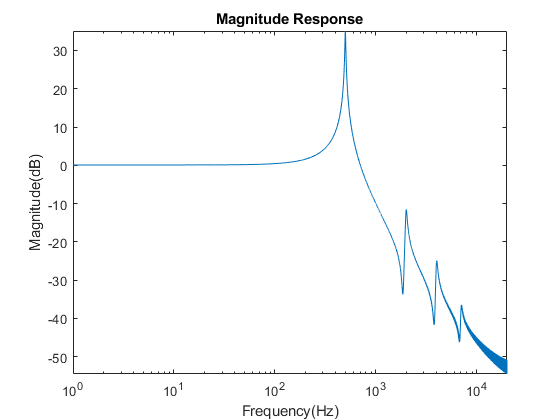
\includegraphics [width=4in]{sysID_m_01.png}
\begin{verbatim}
figure
semilogx(Freq,Phase)
xlabel('Frequency(Hz)')
ylabel('Phase')
axis('tight')
title('Phase Response (radians)')
\end{verbatim}

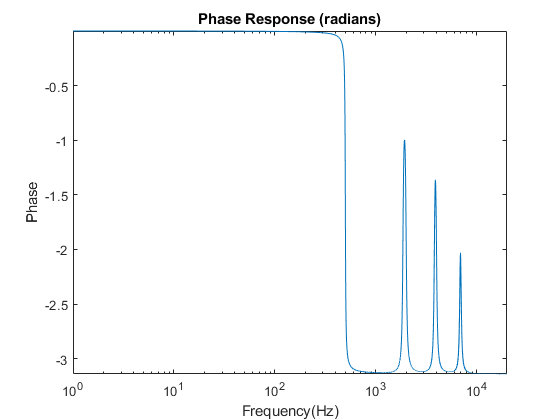
\includegraphics [width=4in]{sysID_m_02.png}
\begin{par}
From the Frequency Response plots, there are 4 resonant modes induced in the system, hence it is modelled as 8 pole and 6 zeros system as a results of the location of the peaks and shalows in the magnitude response.
\end{par} \vspace{1em}
\begin{verbatim}
sys = frd(MagR,Freq*2*pi);
G = tfest(sys,8,6);
\end{verbatim}
\begin{verbatim}
opts = bodeoptions('cstprefs');
opts.PhaseVisible = 'off';
opts.FreqUnits = 'Hz';
semilogx(Freq,20*log10(Mag));
hold on
bodeplot(G,opts,'red');
legend('Nanopositioner ', 'Estimated System','Location','southwest')
\end{verbatim}

        \color{lightgray} \begin{verbatim}Warning: Ignoring extra legend entries. 
\end{verbatim} \color{black}
    
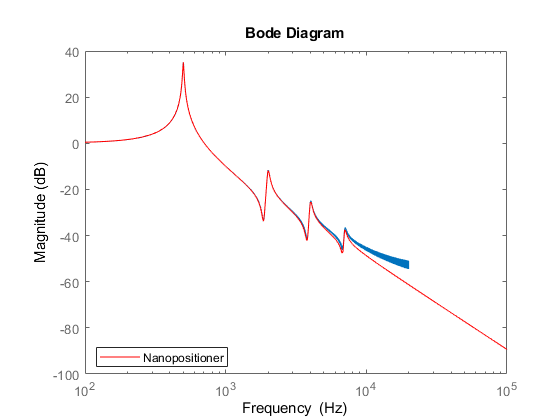
\includegraphics [width=4in]{sysID_m_03.png}
\begin{verbatim}
opts = bodeoptions('cstprefs');
opts.PhaseUnits = 'rad';
opts.MagVisible = 'off';
opts.FreqUnits = 'Hz';
semilogx(Freq,Phase);
hold on
bodeplot(G,opts,'red');
legend('Nanopositioner ', 'Estimated System','Location','southwest')
\end{verbatim}

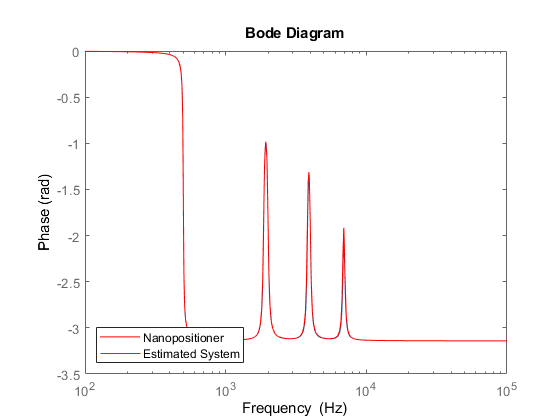
\includegraphics [width=4in]{sysID_m_04.png}
\begin{verbatim}
G % estimated state space system
[r,p,k] = residue(G.Numerator,G.Denominator);
\end{verbatim}

        \color{lightgray} \begin{verbatim}
G =
 
                                                                           
   1.342e07 s^6 + 3.938e10 s^5 + 3.42e16 s^4 + 5.328e19 s^3 + 1.854e25 s^2 
                                                                           
                                                    + 1.088e28 s + 1.928e33
                                                                           
  ---------------------------------------------------------------------------
                                                                             
  s^8 + 3199 s^7 + 2.738e09 s^6 + 4.857e12 s^5 + 1.656e18 s^4 + 1.219e21 s^3 
                                                                             
                                    + 2.091e26 s^2 + 2.136e28 s + 1.905e33   
                                                                             
 
Continuous-time identified transfer function.

Parameterization:
   Number of poles: 8   Number of zeros: 6
   Number of free coefficients: 15
   Use "tfdata", "getpvec", "getcov" for parameters and their uncertainties.

Status:                                                
Estimated using TFEST on frequency response data "sys".
Fit to estimation data: 99.9%                          
FPE: 2.326e-06, MSE: 2.323e-06                         
\end{verbatim} \color{black}
    \begin{verbatim}
[num_1,den_1] = residue(r(1:2),p(1:2),0);
G1 = tf(real(num_1(2)),den_1);
\end{verbatim}
\begin{par}
$$G_{1}(s) = \frac{7.22e05}{s^{2} + 1644s + 1.935e09}$$
\end{par} \vspace{1em}
\begin{verbatim}
[num_2,den_2] = residue(r(3:4),p(3:4),0);
G2 = tf(real(num_2(2)),den_2);
\end{verbatim}
\begin{par}
$$G_{2}(s)= \frac{1.253e06}{s^{2} + 997s + 6.316e08}$$
\end{par} \vspace{1em}
\begin{verbatim}
[num_3,den_3] = residue(r(5:6),p(5:6),0);
G3 = tf(real(num_3(2)),den_3);
\end{verbatim}
\begin{par}
$$G_{3}(s)= \frac{1.578e06}{s^{2} + 502.4s + 1.579e08}$$
\end{par} \vspace{1em}
\begin{verbatim}
[num_4,den_4] = residue(r(7:8),p(7:8),0);
G4 = tf(real(num_4(2)),den_4);
\end{verbatim}
\begin{par}
$$G_{4}(s)= \frac{9.87e06}{s^{2} + 55.29s + 9.87e06}$$
\end{par} \vspace{1em}
\begin{verbatim}
G_comp = G1+G2+G3+G4;
\end{verbatim}
\begin{verbatim}
[num,den] = tfdata(G_comp);
syms s
t_sym = poly2sym(cell2mat(num),s)/poly2sym(cell2mat(den),s);
char = latex(t_sym)
\end{verbatim}

        \color{lightgray} \begin{verbatim}
char =

    '\frac{\frac{3603061052953437\,s^6}{268435456}+\frac{5133228042542267\,s^5}{131072}+34201960011978316\,s^4+53190017306428194816\,s^3+18535717911085316239785984\,s^2+10881908091434080772873519104\,s+1928359649544455558686253089030144}{s^8+\frac{7034612434488761\,s^7}{2199023255552}+\frac{5741166758948537\,s^6}{2097152}+\frac{2486760026298577\,s^5}{512}+1656442354377754880\,s^4+1218871679859894779904\,s^3+209140172229026439596343296\,s^2+21356621499507234816277872640\,s+1904834843397118558787398335987712}'

\end{verbatim} \color{black}
    \begin{par}
$$\frac{\frac{3603061052953437\,s^6}{268435456}+\frac{5133228042542267\,s^5}{131072}+34201960011978316\,s^4+53190017306428194816\,s^3+18535717911085316239785984\,s^2+10881908091434080772873519104\,s+1928359649544455558686253089030144}{s^8+\frac{7034612434488761\,s^7}{2199023255552}+\frac{5741166758948537\,s^6}{2097152}+\frac{2486760026298577\,s^5}{512}+1656442354377754880\,s^4+1218871679859894779904\,s^3+209140172229026439596343296\,s^2+21356621499507234816277872640\,s+1904834843397118558787398335987712}$$
\end{par} \vspace{1em}
\begin{verbatim}
figure
bode(G_comp)
\end{verbatim}

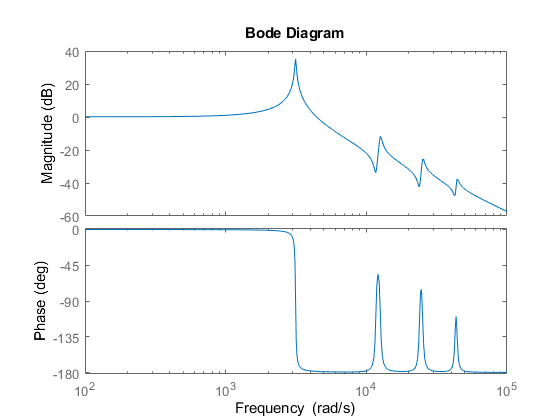
\includegraphics [width=4in]{sysID_m_05.png}
\begin{par}
\textbf{Open Loop Simulation}
\end{par} \vspace{1em}
\begin{verbatim}
T = 2*(1/40);

fs = 44100;
t = 0:1/fs:T-1/fs;

x = 1e-9*sawtooth(2*pi*40*t,1/2);
x_model = lsim(G_comp,x,t);
figure
plot(t,x,t,x_model)
axis('tight')
grid on
ylabel('Displacement (nm)')
xlabel('time (seconds)')
\end{verbatim}

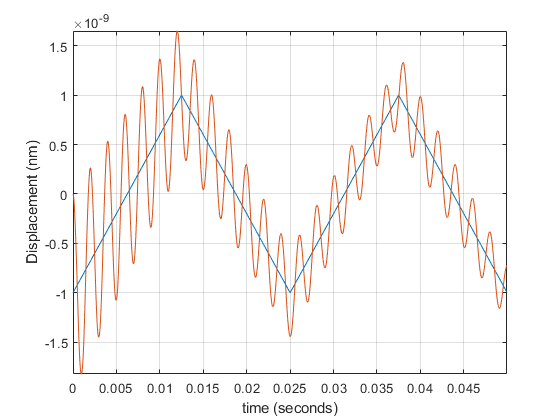
\includegraphics [width=4in]{sysID_m_06.png}
\begin{verbatim}
error = x-x_model';
figure
plot(t,error)
axis('tight')
ylabel('Displacement (nm)')
xlabel('time (seconds)')
\end{verbatim}

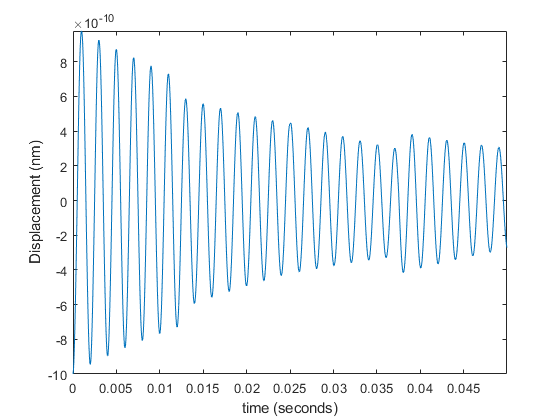
\includegraphics [width=4in]{sysID_m_07.png}



\end{document}

